\subsection{Classic Monte Carlo}
\subsubsection{Theory} \label{sec:classic_mc_theory}
In general monte carlo data are generated if an experiment or an calculation doesn't have sufficient training data. To generate data using the Monte Carlo method we can following these steps (\cite{1905.02666}):
\begin{enumerate}
	\item At first we need a set of random variables $\textbf{X}=\{X_1, X_2, \dots, X_N\}$. In our case this values describe the asset price and other sources of uncertainties.
	\item With this information's we can now create additional information. In our case we can build $M$ random price paths $\{ \textbf{X}_1, \textbf{X}_2, \dots, \textbf{X}_N \}$ .
	\item At the end we want to have the expected value of the payoff $\mathbb{E}_P$, for this we can calculate the payoff of every path $F(\textbf{X}_i)$ and then build the average of the results:
	    \begin{align}
	        \mathbb{E}_P[F(\textbf{X})] = \frac{1}{M} \sum_{i=1}^{M} F(\textbf{X}_i)
	    \end{align}
\end{enumerate}

In this work we will use the "Black-Scholes-Merton" model to create the paths of the stock price. After the Black-Scholes-Merton method the value of the stock changes each step after a log-normal distribution shown in figure \ref{fig:stockPaths}.

To calculate the end result we split the time frame $T$ in $n$ steps, with each step the size of $dt=\frac{T}{n}$. We need also the volatility $\sigma$ and the drift $r$ of the stock.
\begin{figure}[H]
  \begin{center}
    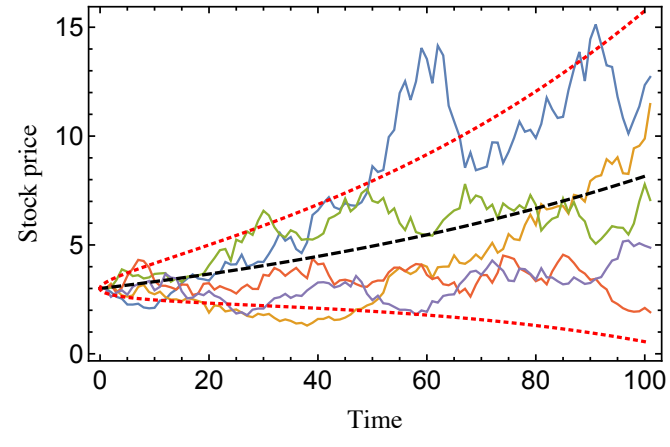
\includegraphics[width=0.5\linewidth]{images/stock_path.png}
  \end{center}
  \caption{Image of five different paths of the stock price. The stock price is in dollar and the time is in days. The dashed black line is the mean of the samples and the dotted red lines are the first standard deviation. The parameters are: $S_0=\$3, r=0.1, \sigma=0.25$ \cite{1805.00109}}
  \label{fig:stockPaths}
\end{figure}
Now $\Pi$ is the true option price and $\hat{\Pi}$ is the approximation of the option price calculated via the Monte Carlo data, with $M$ samples. With this values and the condition that the variance of the payoff function is $ \leq \lambda^2$ the probability that $|\Pi-\hat{\Pi}| \leq \epsilon$ can be determined by Chebyshev’s inequality (\cite{1504.06987}).
\begin{align}
	        P[|\Pi-\hat{\Pi}| \leq \epsilon] \leq \frac{\lambda^2}{M\epsilon^2}
	    \end{align}
So to achieve an error of $\epsilon$
\begin{align}
	        M=\mathcal{O}(\frac{\lambda^2}{\epsilon^2}) \label{eq:classic_M}
	    \end{align}
samples are needed. Section \ref{sec:MC_quanten} shows that quantum computer can improve this from $\epsilon^2$ to $\epsilon$.

\subsubsection{Example} \label{seq:MC_example}
In this subsection a easy Monte Carlo method is shown. Therefor we create only four different stock path and only the last value is of interest, so we get this values:
\begin{align}
    \{\textbf{X}_1=1.5, \textbf{X}_2=2.3, \textbf{X}_3=2.8, \textbf{X}_4=2.11\} \nonumber
\end{align}
We use $S_0=2$ as initial value, $K=2.1$ as strike price and this
\begin{align}
    F(\textbf{X}_i) = \max\{0, X_i - K\} \label{eq:MC_example_european}
\end{align}
as the payoff function. With this kind of information's we can now calculate our expected payoff
\begin{align}
    \mathbb{E}_P[F(\textbf{X})] &= \frac{1}{4}(0+0.01+0.2+0.7 ) \nonumber \\
    &= 0.2275 \nonumber
\end{align}
\bibliography{././refs}